\title{Cocktailmaster 5000}
\team{%
    Robin Aebi,
    Kim Schenk}

\client{Eigenes Projekt}

\projtype{Pro5E}

\coaches{%
    Dr. Prof. Pascal Schleuniger}

\fssummary{
``I drink to make other people more interesting.`` - 
Ernest Hemingway\\

``There can’t be good living where there is not good drinking.`` - 
Benjamin Franklin\\

``Je später der Abend, desto schöner die Gäste.`` - Robin Aebi\\

``Bier macht dick, Schnaps macht krank. Ich bin Kiffer, Gott sei Dank.`` - Kim Schenk\\

    Ob Gartenpartys, Schulfeten oder die ach so wichtigen Networking-Events, eine angemessene Versorgung und Unterhaltung der Gäste ist unerlässlich. Nur steht dabei der eigene Plausch im Hintergrund, und die Kosten für einen Barmann im Vordergrund. Abhilfe schafft hier der Cocktailmaster 5000. Er gibt Ihnen die Möglichkeit, Ihre Zeit für die Unterhaltung und Networking zu nutzen, hält die Personalkosten im Griff und unterhält erst noch die Gäste. Der Cocktailmaster verbindet das Beste aus schon bestehenden Cocktailmaschinen.}

\fsgraphics{
    \begin{minipage}{0.5\textwidth}
        \includegraphics[height=70mm]{images/ender.png}
       % \graphicscaption{Ender 3 Pro}
    \end{minipage}%
    \begin{minipage}{0.5\textwidth}
        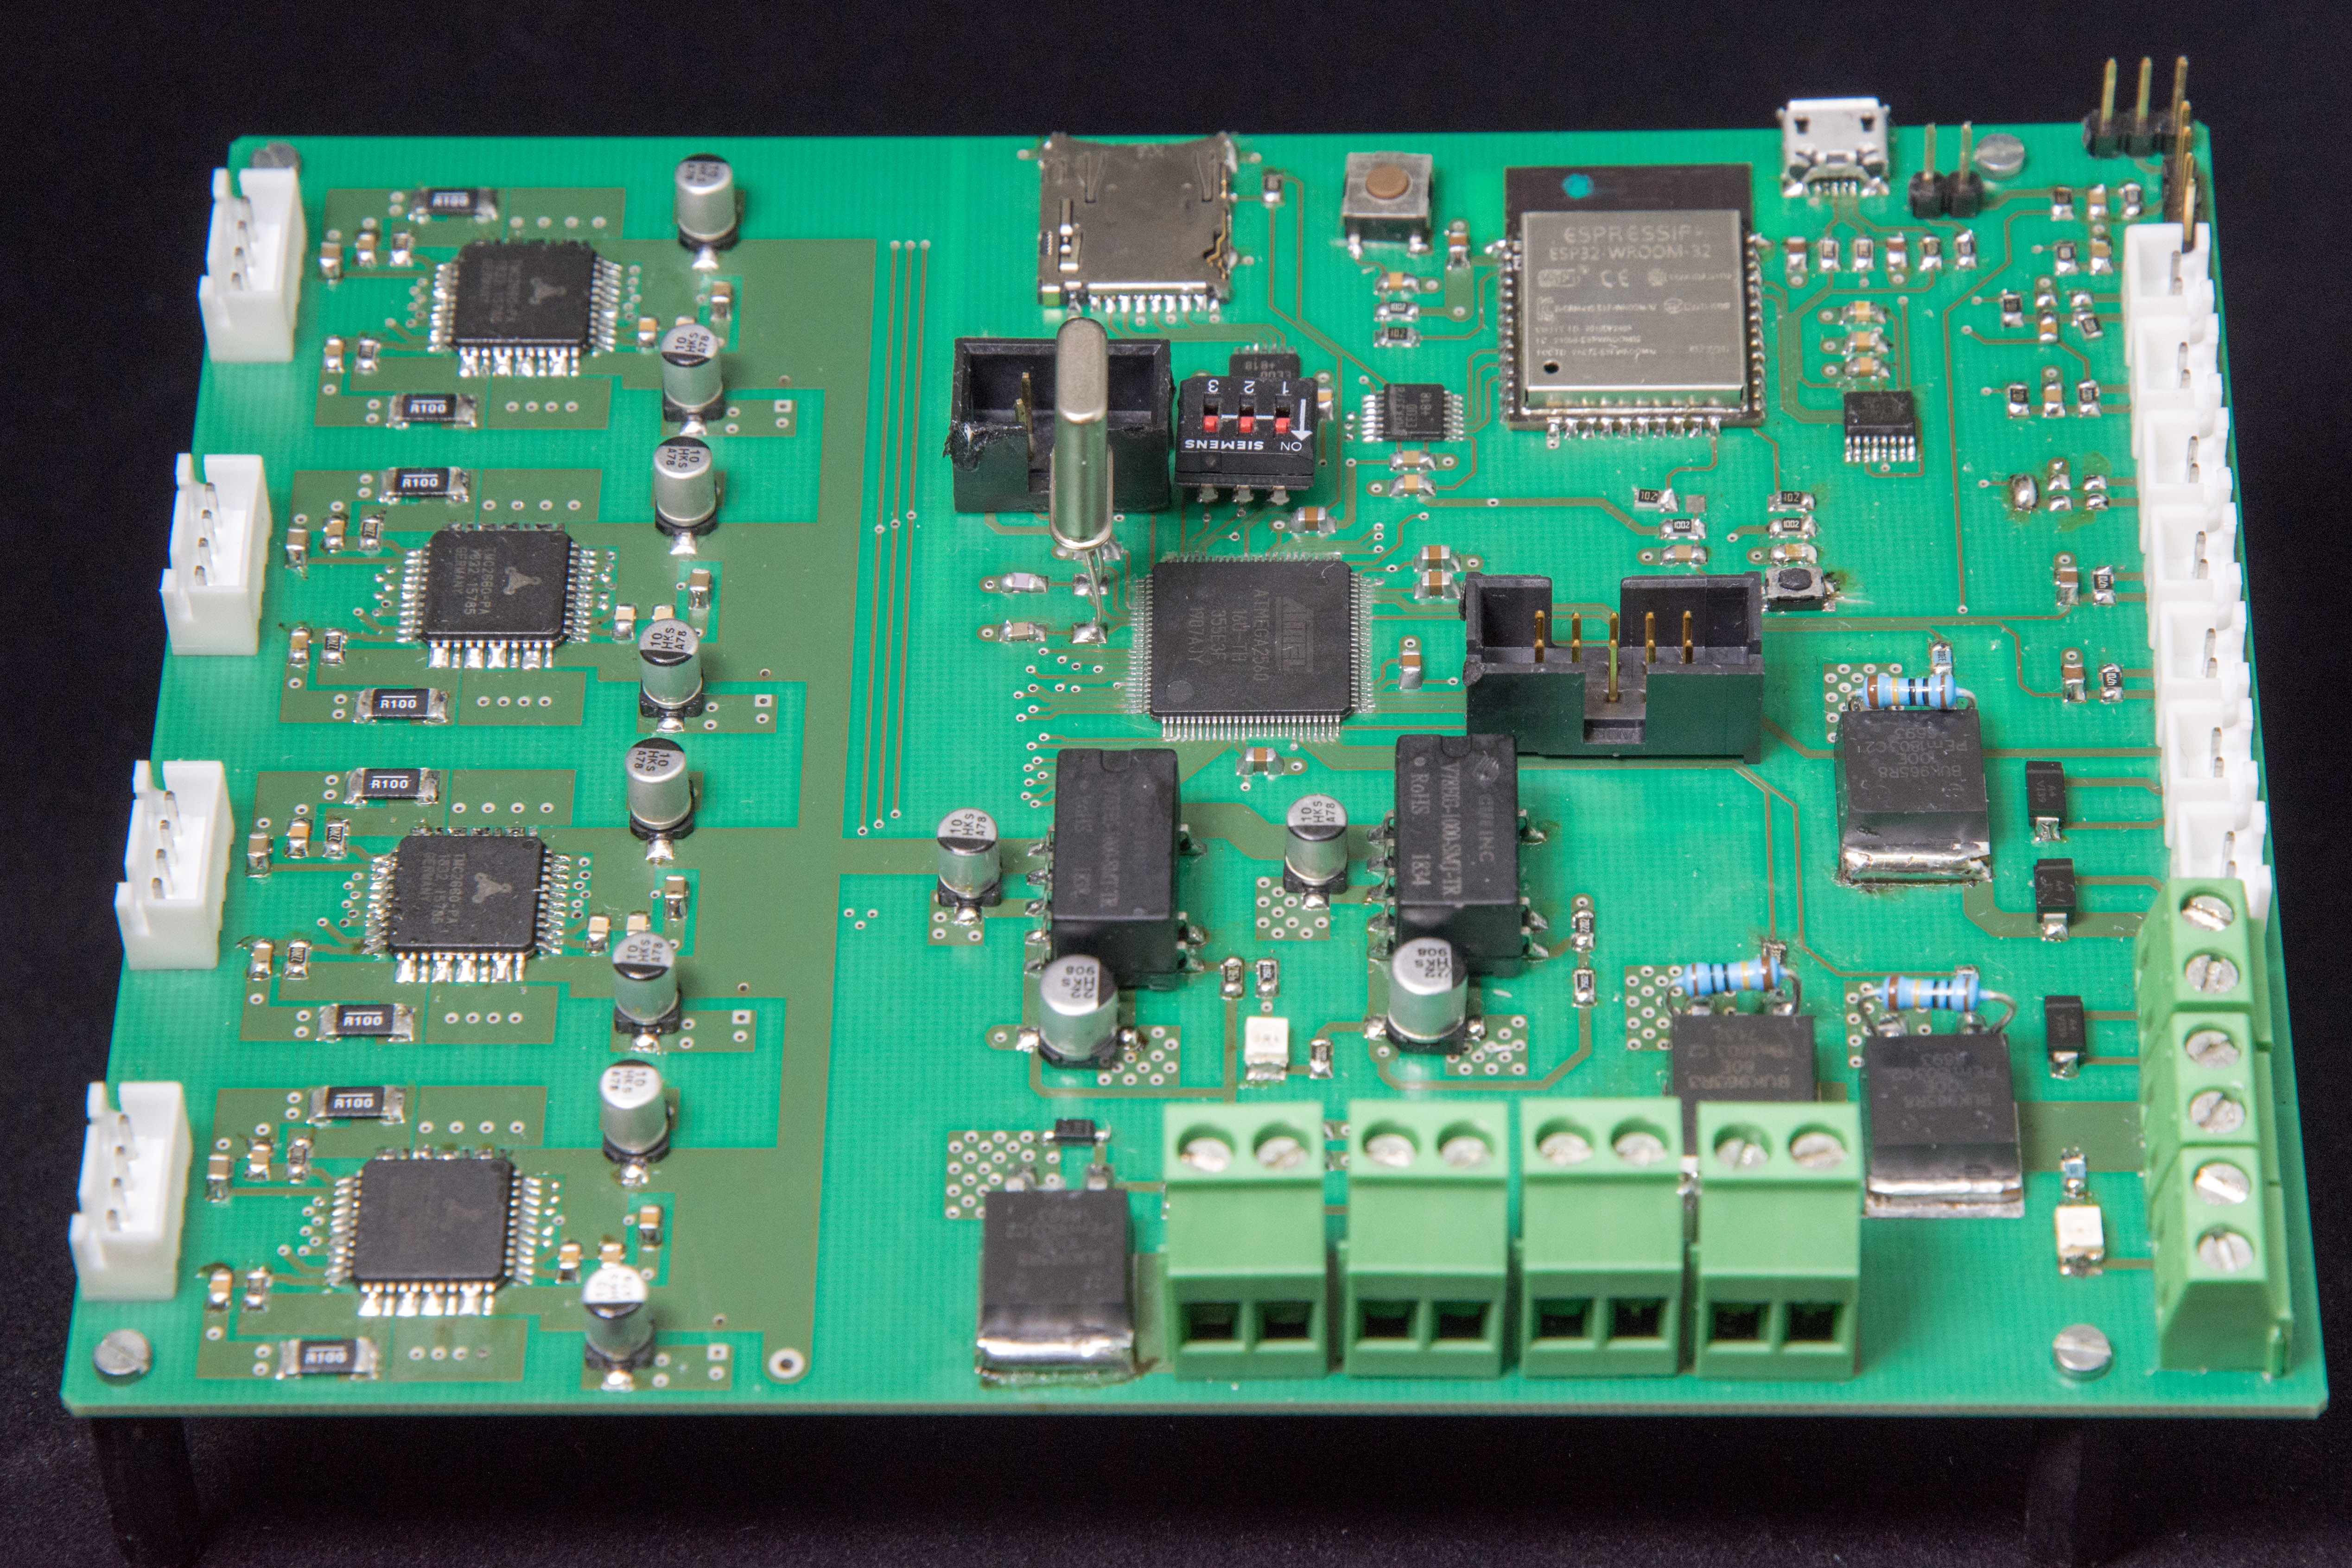
\includegraphics[height=50mm]{images/printplatte.jpg}
        %\graphicscaption{Steuerungsprint}
    \end{minipage}
}

\fscontent{
    \section{3D-Technologie}
    3D-Drucker mit guter Qualität sind sehr teuer. Während der mechanische Teil von günstigen Varianten brauchbar ist, ist die Soft- und Hardware meist fehleranfällig. Die Qualität könnte daher mit einem Hardware und Software Retrofit erheblich verbessert werden. 

    Genau an diesem Punkt setzt der Ender 3 Pro an. Der ursprüngliche Drucker ist preislich auf der günstigen Seite. Die Mechanik des Druckers bietet eine solide Grundlage mit X- und Y-Achse als Riemen-Antrieb und die Z-Achse als Spindel-Antrieb. 
    
    Leider ist es beim Ender nicht möglich per W-Lan auf den Drucker zuzugreifen. Es treten teilweise auch Softwarefehler auf, die den Druck beschädigen können. Sogar die Leistung und die Funktionen der Motorentreiber sind eher gering. All diese Punkte können mit einem Soft- und Hardware Retrofit verbessert werden.

    \section{Ender 3 Pro}
    Der Drucker vom Typ Ender 3 Pro wird mit einer komplett neuen Steuerung ausgerüstet. 
    
    Für die Ansteuerung der Motoren werden neu TMC2660 Motorentreiber von Trinamic verwendet. Dies ermöglicht den Druck schneller und kontrollierter zu fertigen. Weiter ist ein "sensor less homig" möglich. Somit fallen die Endschalter des Enders weg. 
    
    Der Einbau eines ESp32 Moduls bringt den Vorteil, den Drucker über das Wlan-Netz zu erreichen. 
    
    Die Nozzle dient dazu, das Niveau des Heizbetts auszumessen und Schräglagen per Software zu korrigieren.

    \section{Die Bedienung}
   Es gibt zwei Arten, wie der 3D-Drucker bedient werden kann. Die erste Variante beschränkt sich darauf, eine SD-Karte mit dem Druckauftrag zu beschreiben und diese einzusetzen. Der Druck kann mit dem Display gestartet werden.
   
   Die Zweite Art funktioniert über das Programm ESP3D. Auf dieser Webseite ist es möglich Druckaufträge zu verwalten, den Status des Druckers auszulesen und den Ender manuell zu Steuern. \\
   \\
   \begin{minipage}{0.6\textwidth}
   	\includegraphics[height=25mm]{images/ESP3D.png}
   \end{minipage}
}

\infobox{Highlights}{%
    \footnotesize
    \setlength\tabcolsep{2pt}
   	\begin{itemize}
   	\item ATMega 2560 16MHz Taktfrequenz
   	\item ESP 32 Fernzugriff mit TCP/IP auf ESP3D
   	\item E-Mail Benachrichtigungen mit ESP 32 und dem E-Mail Service
   	\item Sensorloses referenzieren mit "StallGuard" von Trinamic
   	\item Automatisches "bed leveling" mit dem PL-touch Sensor
   	\item Filament Sensor erkennt, ob Material vorhanden ist
   	\item Alleinstehender Betrieb
   	\item G-Code files gespeichert mit micro SD-Karte
	\end{itemize}
}
